% !TEX root = ../thesis.tex
%
\chapter{Related Work}
\label{sec:related}
\todo{Just a collection of thoughts for now, needs to be polished a lot}

% \cleanchapterquote{A picture is worth a thousand words. An interface is worth a thousand pictures.}{Ben Shneiderman}{(Professor for Computer Science)}
As Runtime monitoring and verification is a widely researched field, multiple approaches to attain it's goals were developed.

As stated in~\cite{Havelund2008} most approaches are geared towards software written in Java, while many critical systems are written in C and there are countless other systems that could benefit from monitoring and verification written in all kinds of programming languages.
With TeSSLa as a specification Language over Streams, which has no assumptions on the environment of the system that produces the Streams,  as the base for our monitoring approach, we recognized the possibility to abstract the monitoring plattform from the monitored program.
This means that the developed runtime for TeSSLa specifications is not restricted to monitor programs written in a specific language but can monitor anything that can produce Streams.

To show that the runtime is valuable in the context of existing approaches, we will show ways to generate traces from systems that were used to evaluate other monitoring techniques.
Afterwards we will compare the expressiveness of TeSSLa and the runtime with other approaches, based on the generated traces, to show what kinds of specifications can be monitored with TeSSLa and where the Language or the runtime can be extended.

The following Chapter will highlight the systems against which TeSSLa and the runtime is evaluated, furthermore it will also give insights into other work that TeSSLa and this thesis is based on.

\section{TeSSLa}
\label{sec:related:tessla}

The implemented Runtime and the theoretic work of this thesis is built upon the TeSSLa project in~\cite{Decker2016}.
For the project the syntax and a formal semantic of a specification language was defined.

Specifications in TeSSLa are based on streams of data.
Streams are the representation of things that change over time, e.g.\ a variable in a program.
To model streams, TeSSLa defines a timing model.
That model is based on timestamps that are isomorphic to real numbers \(\mathbb{R}\).
Figure~\ref{fig:tessla_streams} shows how streams behave over time.

\begin{figure}\label{fig:tessla_streams}
  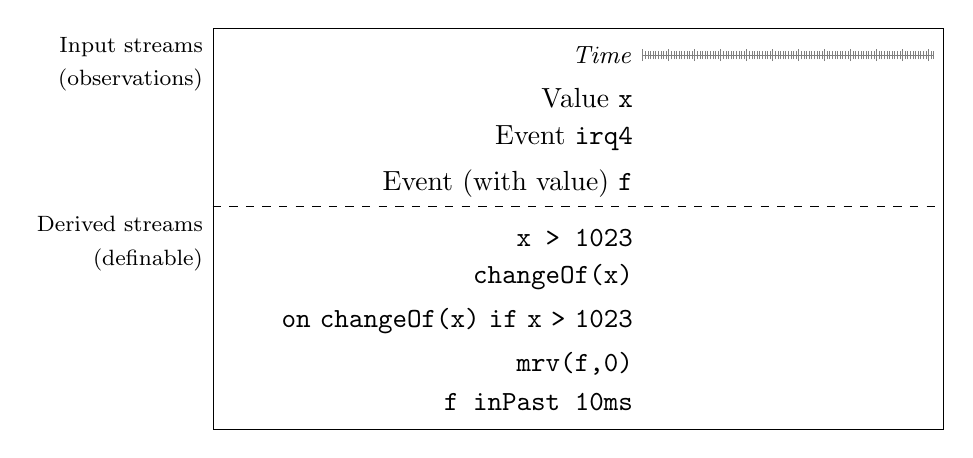
\begin{tikzpicture}

\matrix[column sep = 0.5em, draw] (m) {
  \node[anchor = east] {\small \textit{\textrm{Time}}}; \& \draw[help lines] (0,-0.05) grid[xstep=0.033] (3.7,0.05);
     \draw[gray] (0,-0.075) grid[xstep=0.33] (3.7,0.075); \\[0.5ex]
  \node[anchor = east] (m-1-2) {Value \texttt{x}}; \& \timing[name=m-2-2] at (0,-0.15) {2D{998}N(x1)2D{42}3D{2012}3D{1280}DD{10}DD{1404}};\\
%
  \node[anchor = east] (m-1-3) {Event \texttt{irq4}};
    \& \timing[name=m-2-3] at (0,-0.15) {ZZZ \n{} Z \n{} ZZZZ \n{} ZZ \n{} ZZZ \n{} Z}; \\
%
  \node[anchor = east] (end-inputs) {Event (with value) \texttt{f}};
    \& \timing[name = end-inputs-2] at (0,-0.15) {Z \n{17} ZZZZZZZ \n{98} Z \n{0} ZZZZ \n{23} Z}; \\[0.5em]
%
     \node[anchor = east] (m-1-5) {\texttt{x > 1023}};
  \& \timing[name=m-2-5] at (0,-0.15) {4L 6H 2L 2H}; \\
%
     \node[anchor = east] (m-1-6) {\texttt{changeOf(x)}};
  \& \timing[name=m-2-6] at (0,-0.15) {2Z \n{} 2Z \n{} 3Z \n{} 3Z \n{} 2Z \n{} 2Z}; \\
%
     \node[anchor = east, text width = 14.5em, align = right] (m-1-7) {
          \texttt{\textbf{on} changeOf(x) \textbf{if} x > 1023}};
  \& \timing[name=m-2-7] at (0,-0.15) {4Z \n{} 3Z \n{} 3Z 2Z \n{} 2Z}; \\
%
     \node[anchor = east] (m-1-8) {\texttt{mrv(f,0)}};
  \& \timing[name=m-2-8] at (0,-0.15) {D{0} 7D{17} D{98} 4D{0} D{23}}; \\
%
     \node[anchor = east] (m-1-9) {\texttt{f inPast 10ms}};
  \& \timing[name=m-2-9] at (0,-0.15) {L 2H 5L 3H 2L H}; \\
%
 };

\path[draw, dashed] (m.west|-end-inputs.south) edge (m.east|-end-inputs.south);

\path (m.north west) node[anchor = north east, align = right]
{\footnotesize{Input streams} \\ \footnotesize{(observations)}};

\path (m.west|-end-inputs.south) node[anchor = north east, align = right] {
  \footnotesize{Derived streams} \\ \footnotesize{(definable)}};

\end{tikzpicture}

  \caption{Visualization of TeSSLas Stream model, taken from~\cite{Decker2016}}
\end{figure}

The syntax of TeSSLa specifications is pretty small, but can be used to define complex functions and specifications:

\begin{align*}
  spec \text{ ::= } &\textttbf{define } name[\textttbf{:}\ stype] \textttbf{ := } texpr |\\
                    & \textttbf{out } texpr |
                    spec\ spec\\
  texpr \text{ := } & expr[\textttbf{:}\ type] \\
  expr \text{ := }  & name \mid literal \mid name\textttbf{(}texpr(\textttbf{, }texpr)^*\textttbf{)}\\
  type \text{ := } & btype \mid stype \\
  stype \text{ := } & \textttbf{Signal<}btype\textttbf{>} \mid \textttbf{Events<}btype\textttbf{>}
\end{align*}



\section{LOLA}
\label{sec:related:lola}

The concepts of LOLA~\cite{DAngelo2005} are very similar to the ones of TeSSLa.
Both approaches built upon streams of events.
The biggest difference in the modelation is, that while streams in Lola are based on a discrete model of time TeSSLa uses a continuous timing model.

The specification language of Lola is very small (expressions are built upon three operators) but the expressiveness surpasses Temporal Logics and many other Formalisms \citep{DAngelo2005}.
Expressions in Lola are built by manipulating existing streams to form new ones.
Therefore streams depend on other streams, so they can be arranged in weighted dependency graph, where the weight describes the amount of steps a generated Stream is delayed compared to the parent.

Based on this graph a notion of efficiently monitorable properties is given and an algorithm to monitor them is presented.

TeSSLa takes concepts of LOLA and applies them to a continuous model of time and introduces a language and a rich set of functions that can be applied to streams.
The dependency graph is a core concept of TeSSLa and is used to check if specifications are valid (e.g.\ cycle free) and is also the core concept to evaluate specifications over traces in this thesis.

\section{Distributed Verification Techniques}
\label{sec:related:distributed}

While most implementations of RV systems don't consider or use modern ways of parallelism and distribution and focus on programs running locally, in~\cite{Mostafa2015} a way to monitor distributed programs is given.
To do this distributed monitors, which have to communicate with one another, are implemented.

As stated earlier, the TeSSLa runtime doesn't care about the environment of the monitored program, so it doesn't distinguish between traces from distributed and non distributed programs.
But the runtime itself is highly concurrent and can be distributed easily to many processors or event different computers.
Therefore many of the definitions for distributed monitors can be used to reason about the behaviour of the Runtime.


\section{Copilot}
\label{sec:related:copilot}

The realtime runtime monitor system Copilot was introduced in~\cite{Pike2010}.
Copilot is designed to overcome the shortcomings of existing RV tools in regards to hard-realtime software written in C.

To do so they first define characteristics a monitoring approach has to fullfill to be considered valuable for this domain.
The four principles are:

\begin{description}
  \item[Functionality] Monitors cannot change the functionality of the observed program unless a failure is observed.
  \item[Schedulability] Monitors cannot alter the schedule of the observed program.
  \item[Certifiability] Monitors must minimize the difficulty in re-validating the observed program; in particular, we make it our goal to avoid modifying the observed programs source code.
  \item[SWaP overhead] Monitors must minimize the additional overhead required including size, weight, and power (SWaP).
\end{description}

The monitors follow a sampling based approach, where at specified steps the values of global variables are observed and the monitors are evaluated
on that values.
While sampling based approaches are widely disregarded in RV, because they can lead to both false positives and false negatives,
they argue:

\begin{quote}
  In a hard real-time context, sampling is a suitable strategy. Under
  the assumption that the monitor and the observed program share a global clock and a static periodic schedule, while false positives are possible, false negatives are not.~\cite{Pike2010}
\end{quote}

A special detail of Copilot is that monitors aren't inlined into the program but can be scheduled as independet processes.
The implementation of the TeSSLa runtime in this thesis follows a similar approach: It is a totally independent program,
and therefore also has some of the gains in regard to the specified four characteristics.
Because the runtime works with all kinds of traces, it is insignificant how they are produced:
It can work with traces based on sampling, working in a similar fashion as Copilot, or by actually instrumenting code to generate
traces, which alters the semantics of the program.

% Another shortcoming of inlining monitors is that certified code (e.g., DO-178B for avionics [Inc92]) is common in this domain.
% Inlining monitors could necessitate re-certifying the observed program.

\section{RMoR}
\label{sec:related:rmor}

RMoR is another approach on monitoring C programs.
It does so by transforming C code into an \emph{armored} version, which includes monitors to check conformance to a specification.

Specifications are given as a textual representation of state machines.
The specifications are then interweaved into the programm using CIL~\cite{Necula2002}.
Specifications work on the level of function calls and state properties like \emph{write may never be called before open was called}.
Because Software Developers are often working at the same abstraction level (in contrast to e.g.\ assembler or machine instructions), they can define specifications without having to learn new concepts.
For the TeSSLa runtime support for traces at the same abstraction level (function calls, variable reads and writes) is present and used in most of the tests in Section~\ref{TODO}.

Because RMoR specifications are interweaved into the program, their observations can not only be reported but also used to recover the program or even to prevent errors by calling specified functions when some condition is encountered.
The TeSSLa runtime doesn't support this out of the box, as it's primary purpose is testing and offline monitoring, but in Section~\ref{TODO:Further_WORK} we will look at ways to support this.

% \section{Driver Trace}
% \label{sec:related:drivertrace}
\section{MaC}
% \section{RiTHM}
